\chapter{Fundamentos teóricos} \label{ich:fundamentos_teoricos}

En esta sección introduciremos los \textbf{conceptos teóricos} sobre los que se basará la solución al problema que presentamos en este trabajo. Hablaremos de:

\begin{itemize}
	\item Conceptos básicos sobre el aprendizaje automático: qué es, enfoque supervisado y no supervisado, visión por computador, aprendizaje por la máxima pendiente, función de pérdida, aprendizaje profundo y redes convolucionales.
	\item Codificación de la identidad: \textit{embedding} semántico como principal herramienta para codificar la identidad de forma independiente a la edad y uso de \textit{triplet loss} como función de pérdidad para aprender el \textit{embedding}.
	\item Mejoras técnicas objeto de estudio: introduciremos las mejoras técnicas respecto a la función de pérdida \textit{triplet loss}. \textbf{Estas mejoras son parte central del estudio realizado en este trabajo}. Presentaremos el enfoque \textit{online} de \textit{triplet loss}, la técnica \textit{P-K sampling} para generar \textit{batches} de datos y cómo la elección de los triples definen distintos variaciones en la función de pérdida. Estudiaremos también ciertas mejoras en la función de distancia usada en el \textit{embedding}.
\end{itemize}

\section{Aprendizaje automático}

El aprendizaje automático es una rama de la Inteligencia Artificial, que a su vez es una rama de las ciencias de la computación, dedicada al desarrollo de sistemas que resuelvan ciertas tareas de forma inteligente, en base a cierto criterio para especificar qué entendemos por inteligencia \cite{informatica:libro_europa_IA}. El aprendizaje automático logra resolver las tareas propuestas de forma inteligente a partir de algoritmos y modelos capaces de aprender el comportamiento deseado a partir de un conjunto de datos. Previa a la aparición de estas técnicas y modelos, un experto humano era el que diseñaba e implementaba la solución al problema. En el aprendizaje automático, dados un modelo y un algoritmo de aprendizaje, la solución se aprende a partir de los datos \cite{informatica:libro_europa_IA}.

Este enfoque es muy interesante en ciertos problemas en los que no sabemos cómo diseñar una solución pero disponemos de un gran conjunto de datos de ejemplo. Por ejemplo, consideremos el problema de localizar caras en una imagen. Es realmente complicado diseñar manualmente un algoritmo que resuelva esta tarea, pero es relativamente sencillo generar un conjunto de datos para que un algoritmo de aprendizaje automático genere un modelo que haya aprendido a resolver esta tarea. Otra característica interesante del aprendizaje automático es que tiene la capacidad de mejorar su rendimiento al mejorar la calidad y cantidad de datos de entrenamiento \cite{informatica:paper_que_es_ml}.

\subsection{Aprendizaje supervisado y no supervisado}

Podemos realizar una clasificación de los algoritmos de aprendizaje automático en base a la forma de los datos con los que el modelo aprende el comportamiento deseado, que puede ser representado como:

\begin{equation}
	f(x) = y
\end{equation}

donde $x$ es el dato de entrada, $y$ es la salida deseada y $f$ es el cómputo que realiza nuestro modelo. Consideremos por ejemplo el problema de calcular la edad de una persona a partir de una fotografía de su rostro. Entonces $x$ sería una imagen facial, $y$ la edad de la persona que aparece en la imagen y $f$ el cómputo que realiza el modelo entrenado.

Con esto en cuenta, hablamos de \textbf{aprendizaje supervisado} cuando los datos de entrenamiento están etiquetados, es decir, vienen dados como tuplas (dato de entrada, valor objetivo) o $(x, y)$. Siguiendo el ejemplo anterior, tendríamos un conjunto de datos en los que cada imagen viene acompañada con la edad de la persona que aparece en la imagen. Por otro lado, hablamos de \textbf{aprendizaje no supervisado} cuando los datos de entrenamiento vienen sin etiquetar, es decir, para un valor de entrada $x$ no conocemos cuál es el valor de salida $y$ esperado. En algunos casos, disponemos de otra información asociada a los datos de entrada, a partir de la cual podemos aprender el comportamiento deseado. En otros casos ni siquiera disponemos de esa información adicional.

Nuestra \textbf{solución propuesta forma parte del aprendizaje no supervisado}. Como comentaremos en la \sectionref{isec:base_datos_usada}, trabajamos con conjuntos de imágenes en las que únicamente conocemos la identidad del individuo que aparece en la imagen. Estamos cerca de tener un conjunto de datos propiamente etiquetado, pero faltaría que los datos de entrenamiento fueran dados en la forma asociada a una tarea de búsqueda, es decir, una tupla con la imagen de entrada y la lista con los $n$ mejores resultados para esa imagen.

\subsection{Tarea de aprendizaje y aprendizaje por la máxima pendiente}

Recordemos que buscamos modelar cierto comportamiento que viene representado por:

\begin{equation}
	f(x) = y, \; \forall x \in \mathcal{X}
\end{equation}

donde $x$ es el dato de entrada que vive en el espacio $\mathcal{X}$, $y$ es el valor de salida para esa entrada, y $f$ es nuestra función objetivo. Notar que \textbf{no conocemos $f$}, pues conocer dicha función supone que ya conocemos la solución al problema. Para resolver dicho problema, disponemos de una familia paramétrica de funciones:

\begin{equation}
	\Gamma := \conjunto{f_{\theta}: \; \theta \in \Theta \subseteq \R^N }
\end{equation}

Queremos obtener, a partir de unos datos de entrenamiento $\Omega$, la función de $\Gamma$ que más se parezca a la función objetivo $f$ (desconocida). Para ello necesitamos especificar cómo vamos a medir la similitud de nuestra solución a la función objetivo, y cuál es el algoritmo que optimiza dicha noción de similitud. La primera pieza será la \textbf{función de pérdida}, que toma una función candidata $f_{\theta}$, los datos de entrenamiento $\Omega$ y devuelve el error cometido. Denotaremos a dicha función como $\mathcal{L}(f_\theta, \Omega)$. En caso de que dicha función sea diferenciable respecto a $\theta$, podemos aplicar el \textbf{algoritmo de descenso por la máxima pendiente} o descenso del gradiente. Dicho algoritmo busca minimizar el error de la siguiente forma:

\begin{enumerate}
	\item Toma un valor inicial de $\theta_0 \in \Theta$ en base a algún criterio. Por ejemplo, toma dicho valor inicial aleatoriamente.
	\item Actualiza el valor de los parámetros tal que:
	      \begin{equation}
		      \theta_{i + 1} \leftarrow \theta_i - \eta \nabla \mathcal{L}(f_\theta, \Omega)
	      \end{equation}

	      donde $\eta$ es un factor de escalado al que se le conoce como \textbf{tasa de aprendizaje} o \textbf{\textit{learning rate}}.
	\item Se repite el paso anterior hasta que se cumpla cierta condición de parada. Por ejemplo, hasta que hayamos realizado un número dado de iteraciones, hasta que estemos por debajo de cierto umbral de error o hasta que no mejoremos la función de error en cierto número de iteraciones.
\end{enumerate}

La elección de la tasa de aprendizaje es fundamental a la hora de obtener una buena solución. El descenso del gradiente es un método que se fundamenta en el cómputo del gradiente, y por tanto es de carácter eminentemente local. Un valor muy pequeño de $\eta$ provocará que el proceso quede atascado en mínimos locales rápidamente y que el aprendizaje sea muy lento. Un valor muy alto provocará que los cambios en los parámetros sean demasiado bruscos y que no tengamos la granularidad suficiente para explotar los óptimos (aunque sean locales). Todo esto queda explicado en la \imgref{img:valores_learning_rate}.

\begin{figure}[h]
	\centering
	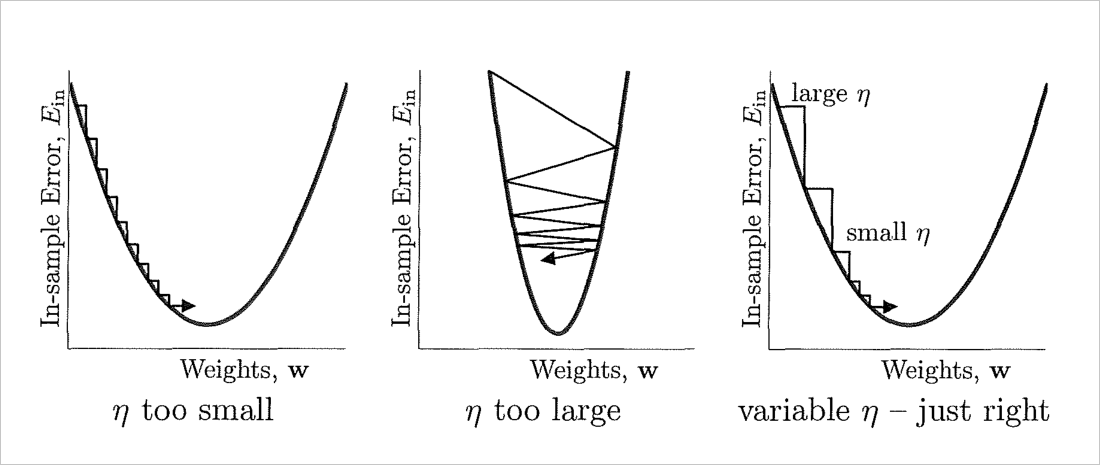
\includegraphics[width=0.8\textwidth]{informatica/valores_learning_rate}
	\caption{Ejemplo gráfico del comportamiento del entrenamiento dependiendo del valor del \textit{learning rate} $\eta$. Imagen extraída de \cite{informatica:libro_clase_aprendizaje_automatico}}
	\label{img:valores_learning_rate}
\end{figure}

\subsection{Descenso del gradiente estocástico}

En el algoritmo del descenso del gradiente hemos actualizado los parámetros de nuestro modelo en base al gradiente de $\mathcal{L}(f_{\theta}, \Omega)$. Esto significa que en una actualización de los parámetros usamos todos los datos de entrenamiento para computar el gradiente, lo que supone algunos problemas. El más evidente es que puede ser computacionalmente muy costoso. Incluso podemos saturar la memoria de nuestro \textit{hardware} al estar trabajando con conjuntos de datos tan grandes. El segundo, al usar todos los datos de entrenamiento para calcular la actualización de los parámetros, podemos estar realizando cambios muy bruscos (porque acumulamos los errores sobre todos los ejemplos de entrenamiento) y poco sutiles (los cambios sutiles que proponen ciertos ejemplos concretos se ven difuminados por el resto de ejemplos). Es por estos dos problemas que se propone el uso del \textbf{descenso del gradiente estocástico}. Dividimos el conjunto de entrenamiento $\Omega$ en subconjuntos $\Omega_i$, $i \in \deltaset{n}$. A estos subconjuntos los llamaremos \textbf{\textit{batches}}. Es claro entonces que:

\begin{equation}
	\Omega = \union_{i = 1}^n \Omega_i
\end{equation}

Con esto, cambiamos ligeramente nuestro algoritmo de aprendizaje, que ahora consistirá en:

\begin{enumerate}
	\item Tomar un valor inicial de $\theta_0 \in \Theta$ en base a algún criterio. Por ejemplo, tomar dicho valor inicial aleatoriamente.
	\item Inicializar $\theta_{k + 1} \leftarrow \theta_k$.
	\item Para cada $i \in \deltaset{n}$, actualizar el valor de los parámetros usando solo información de un \textit{batch}, tal que:
	      \begin{equation}
		      \theta_{k + 1} \leftarrow \theta_{k + 1} - \eta \nabla \mathcal{L}(f_\theta, \Omega_i).
	      \end{equation}
	\item Repetir desde el segundo paso hasta que se cumpla cierta condición de parada. Por ejemplo, hasta que hayamos realizado un número dado de iteraciones, hasta que estemos por debajo de cierto umbral de error o hasta que no mejoremos la función de error en cierto número de iteraciones.
\end{enumerate}

\subsection{Aprendizaje Profundo} \label{isubs:deep_learning_teoria}

El aprendizaje profundo o \textit{deep learning} es una rama del aprendizaje automático caracterizado por el uso de redes neuronales profundas \cite{informatica:paper_deep_learning_def} \cite{informatica:paper_deep_learning_def_second}. Las redes neuronales son modelos que usan unidades más pequeñas llamadas neuronas. Con el paso de los años han aparecido distintos tipos de redes neuronales, en base al tipo de neurona usada. Un primer tipo de red neuronal es el perceptrón multicapa o \textit{MLP}. En esta red la entrada se transforma pasando a través de distintas capa compuestas de varias neuronas que realizan una suma ponderada de las salidas previas, y se aplica una función de activación al valor de dicha suma. La siguiente figura muestra el funcionamiento de una neurona \textit{MLP}:

\begin{figure}[H]
	\centering
	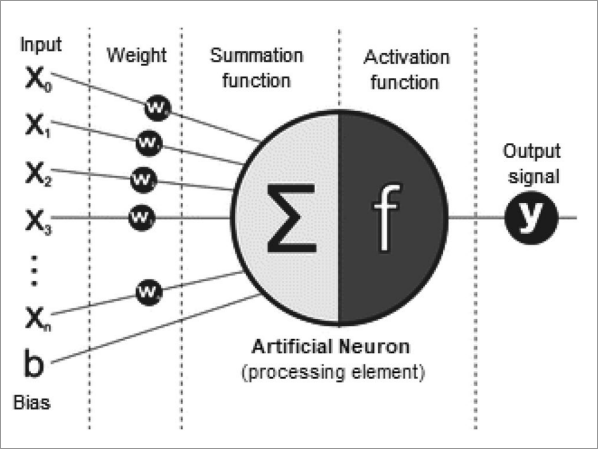
\includegraphics[width=0.4\textwidth]{informatica/neurona_mlp}
	\caption{Ejemplo de cómputo de una neurona en una red neuronal \textit{MLP}. Imagen extraída de \cite{informatica:paper_deep_learning_def}.}
\end{figure}

Las \textbf{redes neuronales profundas} se caracterizan por tener múltiples capas ocultas. Esto es, múltiples capas entre la capa de entrada, que introduce los datos a la red, y la capa de salida, de la que tomamos las predicciones de la red. Este enfoque permite la extracción y representación de características de manera jerárquica, lo que es especialmente útil para tareas de procesamiento de información, como reconocimiento de imágenes, procesamiento de lenguaje natural, traducción automática o procesamiento de voz. El aprendizaje profundo implica que debemos utilizar conjuntos de datos mucho más grandes y que los tiempos de entrenamiento son mucho mayores. Sin embargo, podemos utilizar de forma efectiva dichos conjuntos de datos de gran tamaño, porque estos modelos son más expresivos.

El entrenamiento de estos modelos se realiza con algoritmos basados en el gradiente, como los que hemos introducido o algunas variantes más avanzadas. Actualizar los parámetros del modelo a partir de la información del gradiente de forma directa es computacionalmente muy costoso e ineficiente. El uso del algoritmo de propagación hacia atrás del gradiente o \textbf{\textit{backpropagation}} permite que la optimización de estos modelos con un número tan elevado de parámetros sea factible \cite{informatica:libro_backprop}. La idea clave es actualizar los pesos de las capas más profundas a partir del cálculo del gradiente de forma iterativa, usando la regla de la cadena. Para calcular el gradiente de una capa anterior (menos profunda) usamos el gradiente de la capa posterior (más profunda), y guardamos este cálculo para la siguiente capa anterior. De esta forma aliviamos notablemente la carga computacional.

\subsection{Redes convolucionales}

Las redes convolucionales son un tipo de red neuronal especialmente útiles para trabajar con imágenes. A estas redes se les conoce también como \textit{CNN}, por sus siglas del inglés \textit{Convolutional Neural Networks}. Algunas tareas para las que podemos aplicar estas redes son la clasificación de imágenes o la detección de objetos \cite{informatica:paper_definicion_cnn}. La capacidad de estas redes para aprender representaciones jerárquicas las ha convertido en una de las herramientas más usadas en el ámbito del aprendizaje automático. Estas redes están formadas por los siguientes tipos de capas:

\begin{enumerate}
	\item \textbf{Capas convolucionales}: principal característica de las redes convolucionales. Estas capas están especialmente pensadas para explotar la estructura inherente de las imágenes con las que trabajamos.
	\item Capas de \textit{pooling}: resumen la información para reducir el número de parámetros a optimizar.
	\item Capas totalmente conectadas: capas que toman un vector de entrada y aplican una capa tipo \textit{MLP} (véase la \sectionref{isubs:deep_learning_teoria}).
\end{enumerate}

Desarrollamos en más detalles estas componentes.

\subsubsection{Capa Convolucional}

La capa convolucional es la herramienta que caracteriza este tipo de redes. Esta capa aplica filtros o \textit{kernels} a los datos con los que trabaja, a partir de los cuales extraemos información de dichos datos de entrada. Estos filtros ya se usaban antes de que el aprendizaje profundo se hiciese popular. Sin embargo, dichos filtros eran diseñados manualmente por un experto. En el enfoque del aprendizaje automático los coeficientes de los filtros se aprenden a partir de los datos de entrenamiento.

Estas capas \textbf{explotan eficientemente la estructura de las imágenes} con las que trabajamos. Esta estructura vienen dada por la propiedad de que píxeles cercanos de una imagen (es decir, un vecindario de píxeles) están relacionados entre ellos. Es decir, la posición de un píxel y su vecindario tienen información inherente. Esto queda más claro considerando que si tomamos una imagen y permutamos aleatoriamente sus píxeles, la imagen pierde todo su valor, como hemos mostrado en la \imgref{img:desordenar_pixeles_repetida_mates}.

Podemos aplicar una red \textit{MLP} a imágenes, vectorizando previamente la imagen de entrada (por ejemplo, tomando las columnas de la imagen y concatenando dichas columnas en un único vector). Esto es claramente ineficiente, porque en cada capa combinamos la información de toda la imagen. Para extraer características de la imagen no es útil tomar vecindarios distantes entre sí. Y aquí es donde las capas convolucionales son más eficientes. Estas se basan en el operador matemático de \textbf{convolución}. Dadas dos funciones de variable real, $f$ y $g$, se define su convolución como:

\begin{equation}
	(f * g)(x) := \int f(t) g(x - t) dt.
\end{equation}

Podemos trabajar con una versión discretizada de la convolución, de la siguiente forma:

\begin{equation}
	(f * g)(x) := \sum_{t \in \N} f(t) g(x - t).
\end{equation}

Y a la hora de trabajar con imágenes, que podemos representar como matrices, podemos realizar una convolución discreta entre funciones de dos variables:

\begin{equation}
	(f * g)(x, y) := \sum_{s \in \N} \sum_{t \in \N} f(s, t) g(x - s, y - t).
\end{equation}

Con todo esto ya tenemos las bases matemáticas para implementar una operación que aplique filtros a imágenes de esta forma. Para construir una \textbf{capa convolucional} deberemos fijar los valores de los siguientes hiperparámetros:

\begin{itemize}
	\item Dimensiones del filtro: podemos aplicar un filtro de tamaño $1 \times 1$, en el que en cada paso sólo nos fijamos en un píxel de la imagen. O de tamaño $3 \times 3$, en el que en cada paso nos fijamos en 9 píxeles de la imagen. O cualquier tamaño impar.
	\item Profundidad: cuántos filtros convolucionales se aplican en esta capa. Esto determina cuántas salidas tenemos tras aplicar la capa. A dichas salidas se las conoce como \textbf{mapas de activación}.
	\item \textit{Stride}: tamaño de salto al mover el filtro por la imagen. Podemos aplicar nuestro filtro dando pasos de un píxel, o podemos dar pasos mayores.
	\item \textit{Padding}: Según el tamaño del filtro y el \textit{stride}, podemos tener problemas al llegar a los bordes de la imagen. Podemos aplicar distintas políticas para resolver esto, pero una de las más comunes es ampliar la imagen por cierto tamaño (por ejemplo, copiando los píxeles del borde o usando la media de ciertos píxeles).
\end{itemize}

El funcionamiento de este operador se muestra en la \imgref{img:ejemplo_convolucion}. Esta operación tiene dos propiedades muy relevantes y que justifican su buen funcionamiento. La primera es la \textbf{compartición de coeficientes}. Los coeficientes del operador son independientes de la posición en la que nos encontremos. Si nuestro filtro detecta un patrón, dicha detección debe ser independiente de la posición en la que se encuentre dicho patrón. La segunda es la \textbf{localidad}. El operador toma información de vecindarios de píxeles. Esto es relevante por la estructura local que hemos comentado de las imágenes.

\subsubsection{Capa de \textit{pooling}}

El propósito de esta capa es resumir la información de la imagen (o conjunto de mapas de activación) para obtener datos de menor dimensionalidad. Esto ayuda a que la red sea más ligera, pues al reducir la dimensionalidad de los datos, reduce el número de parámetros que necesitamos ajustar. A partir de la experimentación se piensa que además ayuda a introducir cierta invarianza frente a traslaciones. Hay varias formas de realizar esta operación, así que mencionamos algunas de las más usuales:

\begin{itemize}
	\item \textit{Gobal pooling}: tomamos todos los datos y los resumimos como uno solo, por ejemplo, utilizando la media de todos los valores.
	\item \textit{Max Pooling}: aplicamos un filtro que recorre la imagen de la misma forma que una convolución. Pero en vez de aplicar cierta suma ponderada, toma el máximo de los valores que se están considerando en ese paso.
	\item \textit{Average Pooling}: igual que \textit{max pooling}, pero en vez de tomar el máximo, se toma la media de los valores considerados.
\end{itemize}

La \imgref{img:ejemplos_pooling} explica gráficamente estos tres tipos de \textit{pooling} que acabamos de introducir.

\subsection{Visión por computador}

La \textbf{visión por computador} es una disciplina que busca resolver problemas en base a comprender, interpretar y utilizar información visual. Esto involucra ciertas tareas, como pueden ser la adquisición de imágenes digitales, procesado de imágenes o detección de características \cite{informatica:cv_modern_approach}. Esta disciplina se fundamenta sobre muchas otras áreas del conocimiento, entre ellas, la inteligencia artificial y el aprendizaje automático, la radiometría, ingeniería eléctrica, procesado de imágenes, robótica, realidad aumentada y las ciencias cognitivas.

Es claro que nuestra solución forma parte del área de visión por computador. Buscamos comprender información en forma de imágenes (imágenes de rostros) para resolver una tarea (identificar personas independientemente de los cambios asociados al paso del tiempo). Y es aún más claro que esta solución está en la intersección de la visión por computador y el aprendizaje automático, pues usamos técnicas de aprendizaje automático (principalmente, redes convolucionales) para construir un modelo que comprenda la información de las imágenes para resolver la tarea.

\section{Codificación de la identidad}

Para resolver la tarea, buscamos aprender un modelo que codifique la identidad de las personas que aparecen en imágenes de forma independiente a la edad de dichas personas. Para ello, nuestro modelo deberá aprender un \textit{embedding}, que será la herramienta principal para llevar a cabo la codificación. Por consiguiente, en esta sección definiremos qué es un \textit{embedding} semántico, qué función de pérdida podemos utilizar para que nuestro modelo aprenda dicho \textit{embedding} y cómo se ha aplicado de forma clásica dicha función de pérdida

\subsection{\textit{Embedding} semántico} \label{isec:embeddings}

Un \textbf{\textit{embedding}} no es más que un mapeo desde un cierto espacio $X$ de datos de entrada (en nuestro caso, podemos considerar $X$ como el espacio de imágenes en las que aparecen caras, que a su vez puede verse como cierto $\R^M$) a un espacio vectorial $\R^N$. En la mayoría de los casos la dimensión del espacio de llegada $N$ es menor que la dimensión del espacio $X$. Por consiguiente, buscamos que nuestro modelo aprenda una función

\begin{equation}
	\begin{split}
		f_{\theta}: X & \to \R^N \\
		x & \mapsto f_{\theta}(x).
	\end{split}
\end{equation}

que tomamos de una familia paramétrica de funciones $\{f_{\theta}: \theta \in \Theta \}$. En nuestro problema consideramos la familia de redes convolucionales profundas. Así, $\theta$ estaría compuesto por todos los coeficientes que determinan dicho modelo convolucional, por lo que podemos considerar $\Theta \subseteq \R^M$ donde $M$ es el número de coeficientes del modelo. El criterio para escoger una función u otra de mapeo es que este deberá ser \textbf{semántico}. En el espacio de llegada $\R^N$ tenemos una función de distancia:

\begin{equation}
	\begin{split}
		D: X \times X & \to [0, \infty) \\
		x, y & \mapsto D(x, y)
	\end{split}
\end{equation}

Por ejemplo, la distancia euclídea. Queremos que \textbf{datos semánticamente relacionados en $X$ sean mapeados a vectores en $\R^N$ cercanos} por la distancia que fijemos. Del mismo modo, datos semánticamente distintos deberán ser mapeados a vectores distantes. En nuestro problema la semántica viene dada por la identidad de cada persona. Es decir, dos imágenes están relacionadas semánticamente cuando corresponden a la misma persona (independientemente de la edad con la que aparezcan). Veamos ahora algunos ejemplos en los que podemos solucionar cierto problemas a través del uso de \textit{embeddings}.

\begin{ejemplo}
	Consideremos que queremos computar un \textit{embedding} para representar palabras.

	Este problema es especialmente relevante en el ámbito del lenguaje natural. Esto es así porque, si queremos trabajar con texto usando modelos de aprendizaje automático, deberemos primero convertir dicho texto a una representación numérica \cite{informatica:word_embeddings_survey}. Usar, por ejemplo, el código binario que codifica dicho texto no parece muy buena idea, porque este mapeo no es semántico, y pequeños cambios en una palabra provocan grandes cambios en la representación (podemos pensar que el mapeo es discontinuo, aunque no hayamos definido correctamente qué significa esto). En este caso, queremos que palabras con una semántica parecida se transformen a vectores cercanos. Por ejemplo, la distancia entre los \textit{embeddings} de las palabras \entrecomillado{ciudad}, \entrecomillado{pueblo} debería ser mucho menor que la distancia entre los \textit{embeddings} de las palabras \entrecomillado{papel}, \entrecomillado{odio}. Esta idea se puede visualizar en la siguiente representación:

	\begin{figure}[H]
		\centering
		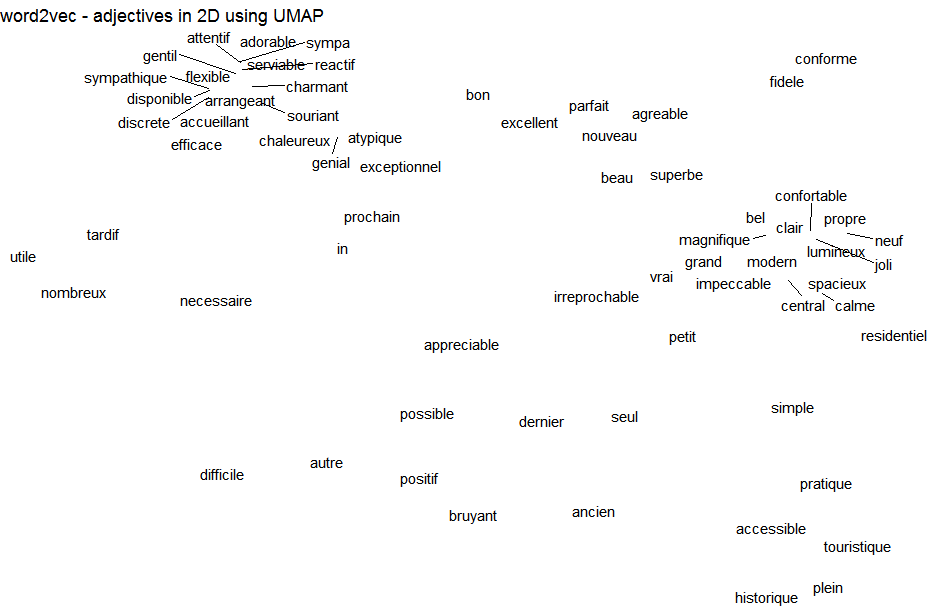
\includegraphics[width=0.6\textwidth]{informatica/word2vec_example}
		\caption{Ejemplo de un \textit{embedding} semántico, computado por el modelo \textit{word2vec} \cite{informatica:word2vec}, de palabras en francés. Imagen extraída de \cite{informatica:word2vec_cran_package}.}
	\end{figure}

	En el caso concreto de \cite{informatica:word2vec}, que propone el conocido modelo \textit{word2vec}, se consigue que el \textit{embedding} tenga cierta \entrecomillado{estructura algebraica}, pudiendo computar, por ejemplo:

	\begin{equation}
		vector("rey") - vector("hombre") + vector("mujer") = vector("reina")
	\end{equation}
\end{ejemplo}

\begin{ejemplo}
	Veamos ahora un ejemplo mucho más cercano con el problema que queremos resolver. Por ejemplo, el problema de re-identificación (ambiente en el que se proponen ciertas técnicas novedosas que estudiaremos más adelante). En este caso, queremos que las imágenes de una persona en una escena, se transformen a vectores cercanos, como muestra la siguiente representación:

	\begin{figure}[H]
		\centering
		\includegraphics[width=0.6\textwidth]{informatica/embedding_paper_principal}
		\caption{Se representa una porción del \textit{dataset} \textit{Market-1501} tras aplicar el \textit{embedding} aprendido y posteriormente \textit{t-SNE}. Imagen extraída de \cite{informatica:principal}}
	\end{figure}

	Por ejemplo, un modelo que quiera resolver esta tarea podría aprender a mapear personas con exactamente la misma ropa a puntos cercanos.
\end{ejemplo}

\begin{ejemplo}

	Y para finalizar, consideremos nuestra tarea en concreto. Buscamos que las imágenes de la misma persona, aunque hayan pasado los años, se transformen en vectores cercanos. Y al contrario, que imágenes de dos personas distintas estén lo más lejos posible.

	Esto es especialmente complicado, como ya hemos comentando en la \sectionref{ich:descrp_problema}, porque por ejemplo, nuestro modelo debe ver como más cercanos imágenes de un niño y un adulto con barba (ambos siendo la misma persona) que dos imágenes de dos adultos con barba (siendo distintas personas). Este problema en concreto lo hemos mostrado en la \imgref{img:ejemplo_dificultad_aifr}.
\end{ejemplo}


\subsection{Redes Siamesas}

Las redes siamesas son redes neuronales que trabajan en paralelo compartiendo los mismos pesos que definen la arquitectura. Normalmente toman dos imágenes de entrada y producen dos vectores de salida de los que se estudia su similitud \cite{informatica:red_siamesa}. Esta forma de trabajar hace que sean una herramienta eficaz a la hora de aprender un \textit{embedding semántico}. Fueron introducidas en \cite{informatica:siamesa_lecunn} para resolver el problema de verificación de firmas manuales. El funcionamiento queda perfectamente explicado en la \imgref{img:siamesa_firma}.

\begin{figure}[!hbtp]
	\centering
	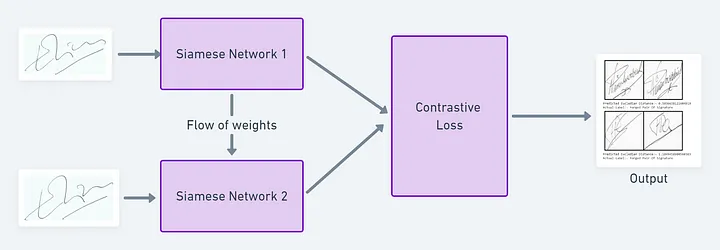
\includegraphics[width=0.9\textwidth]{informatica/siamesa_firma}
	\caption{Ejemplo de funcionamiento de una red siamesa para la verificación de firmas, como planteó \cite{informatica:siamesa_lecunn}. Imagen extraída de \cite{informatica:siamesa_web_imagen}.}
	\label{img:siamesa_firma}
\end{figure}

Para el aprendizaje de las redes siamesas se utiliza principalmente o la función de pérdida \textit{Contrastive Loss} o la función de pérdida \textit{Triplet Loss}. Nuestro trabajo se centra principalmente en \textit{Triplet Loss}, profundizando en las dos variantes \textit{online} objeto de estudio.

\subsection{\textit{Triplet Loss} como función de pérdida para aprender el \textit{embedding}} \label{isec:triplet_loss}

Ya sabemos que para resolver nuestro problema queremos que un modelo convolucional profundo aprenda un \textit{embedding} semántico que codifique la identidad de las personas independientemente de cambios en la edad. Lo que nos falta es una función de pérdida que optimice los parámetros de nuestro modelo. Justificaremos ahora el uso de \textit{triplet loss} como función de pérdida. Recordemos que estamos trabajando con funciones de la forma:

\begin{equation}
	\begin{split}
		f_{\theta}: X & \to \R^N \\
		x & \mapsto f_{\theta}(x)
	\end{split}
\end{equation}

y con una función de distancia:

\begin{equation}
	\begin{split}
		D: X \times X & \to [0, \infty) \\
		x, y & \mapsto D(x, y)
	\end{split}
\end{equation}

Para ser más concisos, usaremos la notación $D_{i, j} := D(f_{\theta}(x_i), f_{\theta}(x_j))$. Como su nombre indica, \textit{triplet loss} trabajará sobre triples. Esto es:

\begin{enumerate}
	\item Una imagen de un individuo concreto, a la que llamaremos \textbf{\textit{anchor}} o ancla.
	\item Otra imagen distinta, pero del mismo individuo, a la que llamaremos \textbf{positiva}.
	\item Una imagen de un individuo distinto, a la que llamaremos \textbf{negativa}.
\end{enumerate}

En este caso, queremos que la distancia entre el \textit{embedding} del ancla y el \textit{embedding} de la positiva (que podemos denotar como $D_{A, P}$) sea mucho menor que la distancia entre el \textit{embedding} del ancla y el \textit{embedding} de la negativa (denotamos $D_{A, N}$). Por tanto, lo que realmente queremos es que:

\begin{equation}
	D_{A, P} \leq D_{A, N}
\end{equation}

o lo que es lo mismo,

\begin{equation}
	D_{A, P} - D_{A, N} \leq 0.
\end{equation}

Una forma trivial de hacer que esa ecuación se cumpla, es haciendo que

\begin{equation}
	f(x) = \vec{0}; \dspace \forall x \in X
\end{equation}

con lo que obtendríamos un modelo totalmente inservible. Para evitar eso, introducimos un término $\alpha > 0$ que se conoce como \textbf{margen}, llegando a:

\begin{equation}
	D_{A, P} - D_{A, N} + \alpha \leq 0.
\end{equation}

Buscamos que el término de la izquierda sea lo más negativo posible, por lo buscamos minimizar la siguiente función de pérdida:

\begin{equation} \label{ieq:triplet_loss_single_entry}
	\begin{split}
		\mathcal{L}_{tri}(\theta; A, P, N) & := max \{D_{A, P} - D_{A, N} + \alpha, 0 \} \\
		&= ReLU(D_{A, P} - D_{A, N} + \alpha).
	\end{split}
\end{equation}

Minimizando esta función de pérdida, lo que haremos será atraer elementos de la misma clase entre sí, y alejar elementos de clases distintas. Este proceso se refleja en la siguiente imagen:

\begin{figure}[H]
	\centering
	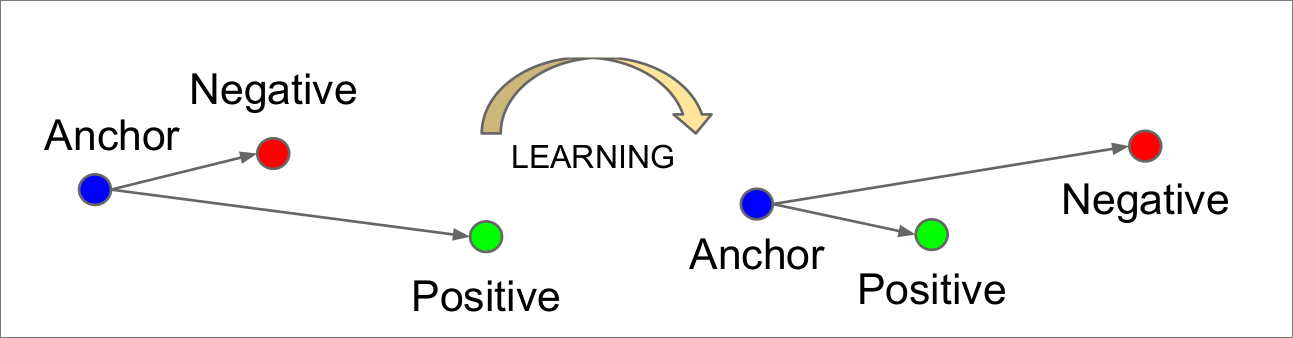
\includegraphics[width=1.0\textwidth]{informatica/triplet_loss_learning}
	\caption{Ejemplo gráfico del proceso de aprendizaje deseado con \textit{triplet loss}. Imagen creada a partir de datos de \cite{informatica:cacd_dataset} en base a \cite{informatica:facenet}.}
\end{figure}

Notar que en \eqref{ieq:triplet_loss_single_entry} trabajamos con una sola entrada de tres datos en forma de imagen. A diferencia de un \textit{dataset} con los datos etiquetados de la forma (entrada, valor de etiqueta), tenemos datos de la forma (imagen, identificador de individuo, edad). Esto supone un problema a resolver: cómo generamos \textit{batches} con triples de la forma (ancla, positivo, negativo) para poder aplicar \eqref{ieq:triplet_loss_single_entry}. Explicaremos cómo solucionar esto en la \sectionref{isubs:enfoque_offline_minado_triples}.

Pero ahora veamos las \textbf{ventajas} que plantea este enfoque. La principal es que, a diferencia de otros enfoques basados en usar funciones de pérdida auxiliares (y que suelen forzar que la red solo pueda funcionar comparando pares de imágenes), el cómputo del \textit{embedding} es directo usando esta función de pérdida (\textit{end to end learning}). Optimizamos directamente la propiedad semántica del \textit{embedding} que deseamos obtener. Una vez entrenado el modelo es directo adaptar el modelo a tareas de \textit{clustering}, \textit{retrieval} o verificación \cite{informatica:principal}. En el \sectionref{isubs:impl_retr_adapter} mostramos lo sencillo que es realizar esta adaptación.

\subsubsection{Minado de triples \textit{offline}} \label{isubs:enfoque_offline_minado_triples}

Como ya hemos comentado, la tarea que debemos resolver ahora es la de generación de \textit{batches} adecuados para poder emplear \eqref{ieq:triplet_loss_single_entry} como función de pérdida a minimizar. Por tanto, dado un conjunto de datos de la forma (imagen, identificador, edad), debemos obtener un conjunto de datos de la forma (img. ancla, img. positivo, img. negativo). Este último conjunto de datos puede ser una lista de triples o un conjunto de \textit{batches}. Como buscamos trabajar con \textit{batches}, en el caso de tener una lista de triples, podemos simplemente muestrear aleatoriamente y sin remplazo de dicha lista, repitiendo el muestreo tras cada época completada.

El \textbf{minado de triples \textit{offile}} es el enfoque clásico que se ha venido usando previo a \cite{informatica:facenet}, trabajo que introduce un enfoque \textit{online} que luego otros trabajos como \cite{informatica:principal} han ido mejorando. Para entender este minado veamos el ciclo de aprendizaje, que se divide en \textbf{varios pasos}. En primer lugar, se realiza el minado \textit{offline} de los triples. Es decir, se obtiene una primera lista o conjunto de \textit{batches} de la forma \lstinline{(img. ancla, img.positivo, img.negativo)}. Una forma de hacer esto sería, por ejemplo, generar los triples de forma aleatoria o generar todos los posibles triples. Aunque estas ideas no suelen funcionar en la práctica. Otra forma más efectiva es seleccionar los triples en base a algún estudio estadístico o usar la red que vamos a optimizar para identificar aquellos triples en los que tiene más dificultad. En segundo lugar, realizamos el aprendizaje sobre dicho conjunto de triples. En algunos casos, realizamos el entrenamiento completo sobre dicho conjunto inicial. En otros casos, principalmente cuando usamos la red para el minado de triples, pasadas algunas épocas de entrenamiento volvemos a generar otra vez la lista de triples. Así, triples que antes la red no identificaba propiamente, ahora sí que los identifica (\entrecomillado{network snapshots}, \cite{informatica:facenet}) y podemos buscar triples más interesantes.

Una vez computado una lista de triples $(a, p, n) \in \Omega$, la función de pérdida \eqref{ieq:triplet_loss_single_entry} se implementa de forma natural como en cualquier otro ámbito de \textit{batching}:

\begin{equation}
	\mathcal{L}_{tri}^{offline}(\theta; \Omega) := \frac{1}{\#\Omega} \sum_{(a, p, n) \in \Omega} \mathcal{L}_{tri}(\theta; a, p, n).
\end{equation}

En la literatura sobre aprendizaje automático normalmente se ignora el término $\frac{1}{\#\Omega}$ y se supone que siempre estamos dividiendo por el número de sumandos, con lo que nuestra función de error suele escribirse como:

\begin{equation}
	\mathcal{L}_{tri}^{offline}(\theta; \Omega) := \sum_{(a, p, n) \in \Omega} \mathcal{L}_{tri}(\theta; a, p, n).
\end{equation}

\subsubsection{Problemas del minado \textit{offline}}

El minado de triples \textit{offline} supone una serie de problemas:

\begin{itemize}
	\item Estamos dividiendo el proceso de aprendizaje en dos etapas, la de minado de triples y la de aprendizaje sobre estos triples. Esto añade complejidad a nuestra \textit{pipeline} (véase la \sectionref{isec:pipeline}).
	\item La adecuada elección de triples es fundamental. Si elegimos triples demasiado fáciles, la red no aprenderá nada nuevo, pues es muy fácil distinguir los ejemplos presentados. Sin embargo, si solo mostramos triples complicados, el modelo se centrará en aprender ejemplos extraordinarios y no sabrá distinguir el grueso de ejemplos más sencillos. Además, generalmente los modelos aprenden rápidamente a distinguir la mayoría de ejemplos en los que las diferencias son relativamente evidentes. Por tanto, en pocas iteraciones la mayoría de triples generados de forma \textit{offline} son demasiado sencillos, lo que agrava mucho el problema que hemos comentado.
	\item Sería conveniente disponer de alguna forma de ajustar la complejidad de los triples presentados. Podemos confiar en que al ir re-generando la lista de triples, la complejidad vaya aumentando. Pero el algoritmo de minado debería tener alguna forma de controlar el énfasis que se hace en la búsqueda de combinaciones difíciles, lo que añade aún más complejidad al sistema.
	\item El minado supone realizar un proceso de búsqueda, que es muy lento (evaluar de alguna forma todos los posibles triples supondría al menos $O(n^3)$). Lo ideal sería disponer de algún método que se basará en muestrear aleatoriamente de nuestra lista de elementos de la forma \lstinline{(imagen, identidad, edad)} (proceso que es muy rápido) y generar triples interesantes sobre dicho muestreo. Esto motiva la técnica introducida en la \sectionref{isubs:triples_online}.
\end{itemize}
